\documentclass[twocolumn]{article}
\usepackage[utf8]{inputenc}
\usepackage{amsmath}
\usepackage{amsfonts}
\usepackage{graphicx}
\usepackage{url}
\usepackage{hyperref}

\title{eQuilibrator 3.0}
\author{Elad Noor, Moritz Emanuel Beber}
\date{October 2019}

\newcommand{\Gmat}{\mathcal{G}}
\newcommand{\PRmat}[1]{P_{\mathcal{R}\left(#1\right)}}
\newcommand{\PNmat}[1]{P_{\mathcal{N}\left(#1\right)}}

\begin{document}

\maketitle

\section{Introduction}
Although thermodynamic theory has been very well established for centuries, and countless examples of its usefulness exist, it seems to be relatively underused in metabolic modeling. A few of the reasons for this are:
\begin{itemize}
    \item \textbf{The knowledge gap} -- equilibrium constants for most biochemical reactions have not been measured.
    \item \textbf{The complexity gap} -- thermodynamic constraints tend to make metabolic models more complicated. For example, FBA with thermodynamic constraints turns from a standard LP to an MILP \cite{henry_thermodynamics-based_2007}.
    \item \textbf{The motivation gap} -- it is not clear to everyone that using thermodynamics in models is actually necessary or even useful.
    \item \textbf{The software gap} -- adding thermodynamics to an existing model requires quite a bit of work (mapping IDs, adjusting the $\Delta G'^\circ$ values to the aqueous conditions, annotating charged molecules correctly).
\end{itemize}

One of the major breakthroughs in bridging the knowledge gap was achieved by Lydersen in 1955, who suggested to adapt the Group Contribution method to the world of organic chemistry, and decades later implemented by Joback and Reid \cite{joback_estimation_1987}, and Mavrovouniotis \cite{mavrovouniotis_group_1988, mavrovouniotis_group_1990}. This data-driven approach was able to cover the majority of the small molecules which appear in metabolic models and obtain estimates for their Gibbs energy of formation \cite{feist_genomescale_2007}. Since then, improvements to the accuracy and coverage of this method have been  \cite{jankowski_group_2008, noor_integrated_2012, noor_consistent_2013, du_temperature-dependent_2018}. It is therefore arguably safe to say that the knowledge gap has been addressed.

Similarly, the complexity gap has changed from an impossible barrier to a small inconvenience, thanks to the incredible progress in the availability of computing power. Beyond the effects of Moore's law, powerful MILP solvers (such as IBM's \href{https://www.ibm.com/products/ilog-cplex-optimization-studio}{CPLEX} and \href{https://www.gurobi.com/}{Gurobi}, which offer free academic licenses) made it as easy as ever to solve large problems that would probably be out of reach only one decade ago (with the same budget).

The motivation gap is harder to overcome, due to a chicken-and-egg problem. Since other, more technical, issues were holding thermodynamic models back -- it was quite difficult to demonstrate the use of these models in reality and therefore convince the scientific community that they are worth investing in. Nevertheless, quite a few algorithms were suggested, which take advantage of such models. Specifically, ways to impose thermodynamic constraints on stoichiometric models were proposed by several different groups \cite{holzhutter_principle_2004,henry_thermodynamics-based_2007,noor_pathway_2014}. These algorithms have the potential to improve the flux predictions produced by flux balance analysis (FBA) \cite{noor_removing_2018}, and assist in the design of new metabolic pathways \cite{hadicke_optmdfpathway:_2018}.

In seems that the time has come to close the last remaining gap, namely the software gap. In recent years, tools such as the COBRA toolbox, COBRApy, ModelSEED, Escher, and Memote, have facilitated the use of genome-scale metabolic models and made them an industry standard which is applied in thousands of scientific projects every year. In 2012, we built the first version of a website called eQuilibrator, which aims to do the same for thermodynamic parameters \cite{flamholz_equilibratorbiochemical_2012}. eQuilibrator provides a simple search-focused interface for quickly finding a biochemical reaction's Gibbs free energy change, and is now used by $\sim$1000 distinct users every month. However, eQuilibrator was never intended to be used for large lists of chemical formulas and therefore does not support a batch mode. In this paper, we highlight the major changes and improvements to the eQuilibrator website, and describe a new Python package (called \textit{equilibrator-api}) which is aimed at novice and expert programmers that want to add thermodynamic parameters to their genome-scale models.


\section{Results}

\subsection{New features in eQuilibrator 3.0}

\subsubsection{The Component Contribution method}
When eQuilibrator was first launched, the $\Delta_r G$ estimates were based on the pseudo-isomeric group contribution method \cite{noor_integrated_2012}. About two years later, we updated the back-end engine to the more recent component contribution (CC) method \cite{noor_consistent_2013}, which required developing a way to calculate CC estimates on-the-fly. In section \ref{sec:on_the_fly} we present for the first time the basis for these calculations. Another advantage provided by the new system, and which can be accessed by our python package, is the full uncertainty co-variance matrix of multiple estimates. It is important to note, that in some cases $\Delta_r G$ estimates can have large uncertainties, but these might be highly correlated between reactions in the model. The full uncertainty can help describe these errors more precisely in high dimension and make a significant difference in some applications, for example when sampling the parameter space. In section \ref{sec:multivariate} we explain how the full co-variance matrix can be used in sampling or in constraint-based thermodynamic models.

\subsubsection{Complete code refactoring}
We have redesigned the entire component-contribution package in a new repository \url{https://gitlab.com/elad.noor/component-contribution}, and integrated it completely into a large framework denoted \textit{eQuilibrator} (see Figure \ref{fig:eq3_design}).

\begin{figure*}
    \centering
    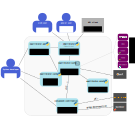
\includegraphics[width=\textwidth]{equilibrator_3_0.pdf}
    \caption{The design of the eQuilibrator 3.0 suite}
    \label{fig:eq3_design}
\end{figure*}

\subsubsection{Support for multiple compound databases}
MetaNetX, KEGG, ChEBI, BiGG, Swiss Lipids (see Figure \ref{fig:eq3_design}).

\subsubsection{Automatic annotation of COBRA models with standard Gibbs free energy values}
\textbf{Needs to be implemented first.}

\subsection{Fast Calculation of Gibbs energies using Component Contributions}\label{sec:on_the_fly}

It is a specific challenge to use the Component Contribution (CC) method in a website such as eQuilibrator, since uncertainty calculations must be made on-the-fly, but the math for CC was developed as a one-step calculation for thousands of reactions in a model. The time it takes to run CC even for a single reaction is too long to be useful for a website.

Therefore, we need to come up with a pre-processing scheme which will probably involve several intermediate matrices in-memory and the remaining calculations will be minimal.

\subsubsection{Standard Component Contribution}\label{sec:standard_cc}
According to the standard CC method \cite{noor_consistent_2013}, the estimated standard Gibbs energies, which is vector denoted by $\Delta_{r}G_{cc,X}^{\circ}$, is given by the formula
\[
X^{\top} \left[ 
\underbrace{\PRmat{S} \left(S^{\top}\right)^{+}}_\textrm{RC} ~+~ 
\underbrace{\PNmat{S^\top} \Gmat \left(S^{\top}\Gmat\right)^{+}}_\textrm{GC}
\right] \Delta_{r}G_{obs}^{\circ}
\]
where $X$ is the stoichiometric matrix of the set of reactions we wish to estimate, $S$ is the stoichiometric matrix of the training data-set, $\Gmat$ is the group incidence matrix, and $\Delta_{r}G_{obs}^{\circ}$ are the observed chemical Gibbs energies of the training set reactions. The orthogonal projections $P_{\mathcal{R}\left(S\right)}$ and $P_{\mathcal{N}(S^{\top})}$ are the projections on the range of $S$ and the null-space of $S^\top$ respectively. The $()^{+}$ sign represents the matrix pseudo-inverse. As indicated by the braces under the two parts, we can separate the contributions to two: Reactant Contributions (RC) and Group Contributions (GC).

The full co-variance matrix of the uncertainty in these Gibbs energies (denoted $\Sigma_{cc,X}$) is given by:
\begin{align}
X^{\top} \left[ \alpha_{rc}\cdot C_{rc} + \alpha_{gc}\cdot C_{gc} + \infty\cdot C_{\infty}  \right] X \label{eq:full_u}
\end{align}
where
\begin{align*}
\alpha_{rc} &\equiv \frac{||e_{rc}||^{2}}{n-\mbox{rank}(S)} \\
\alpha_{gc} &\equiv \frac{||e_{gc}||^{2}}{n-\mbox{rank}(S^{\top}\Gmat)} \\
C_{rc} & \equiv \PRmat{S} \left(SS^{\top}\right)^{+} \PRmat{S} \label{eq:c_rc}\\
C_{gc} & \equiv \PNmat{S^\top} \Gmat \left(\Gmat^{\top}SS^{\top}\Gmat\right)^{+} \Gmat^{\top} \PNmat{S^\top} \\
C_{\infty} & \equiv \Gmat \PNmat{S^\top\Gmat} \Gmat^{\top}
\end{align*}
and $e_{rc}$ and $e_{gc}$ are the residuals of the reactant and group contribution regressions.

Note that the diagonal values in $\Sigma_{cc,X}$ are the squared standard errors of the estimates of single reactions.


\subsubsection{Calculating Gibbs energy estimates on-the-fly}

What happens when we want to estimate the Gibbs energy of reactions with reactants that are not in $S$? The long way would be to augment $S$, $\Gmat$ and $X$ with more rows that would correspond to the new compounds. Note that if we do not have a group decomposition of one of these new compounds, there is no way to make the estimation (we cannot add ``group columns'' like we did for compounds in the training set). Fortunately, we will soon see that the effect of the added rows on the calculation is minimal, and it is easy to do the pre-processing trick we need.

Let $\Gmat'$ be the group incidence matrix of only the new compounds, and $X'$ the stoichiometric coefficients of the new compounds. Then the new matrices we need to use for CC are:

\begin{align*}
	\bar{X} & \equiv \begin{bmatrix} X \\ X' \end{bmatrix} \\
	\bar{S} & \equiv \begin{bmatrix} S \\ 0 \end{bmatrix} \\
	\bar{\Gmat} & \equiv \begin{bmatrix} \Gmat \\ \Gmat'\end{bmatrix}
\end{align*}
It is easy to see that $\bar{S}^\top \bar{\Gmat} = S^\top \Gmat$. Since we added only zeros to $S$, the range will not change, and the null-space of $S^\top$ will include all the new rows. Therefore
\begin{align}
	\PRmat{\bar{S}} & \equiv \begin{bmatrix}\PRmat{S} & 0 \\ 0 & 0 \end{bmatrix}  \\
	\PNmat{\bar{S}^\top} & \equiv \begin{bmatrix} \PNmat{S^\top} & 0 \\ 0 & I \end{bmatrix}
\end{align}

So, the RC term will not change at all, while the GC term can be rewritten in block-matrix form:
\begin{align}\label{eq:P_N_ST_G}
\bar{X}^\top \PNmat{\bar{S}^\top} \bar{\Gmat} &=
\begin{bmatrix} X \\ X' \end{bmatrix}^\top \begin{bmatrix} \PNmat{S^\top} & 0 \\ 0 & I \end{bmatrix}
\begin{bmatrix} \Gmat \\ \Gmat'\end{bmatrix} \nonumber\\
 &= \begin{bmatrix}X^\top \PNmat{S^\top} \Gmat \\ X'^\top \Gmat' \end{bmatrix}
\end{align}

Therefore, when we combine both RC and GC, the upper blocks will sum up to the same value of $\Delta_{r}G_{cc,X}^{\circ}$ before we added $X'$, and the bottom blocks will add a new term, namely:
\begin{align}
    \Delta_{r}G_{cc,\bar{X}}^{\circ} = \Delta_{r}G_{cc,X}^{\circ} + X'^\top \Gmat' \left(S^{\top}\Gmat\right)^{+} \Delta_{r}G_{obs}^{\circ}
\end{align}

Finally, we can define the pre-processing vectors (which depend only on the training data and not on the reaction we wish to estimate) as:
\begin{align*}
	v_{r} &\equiv
	\left[
		\PRmat{S} \left(S^{\top}\right)^{+} + 
		\PNmat{S^\top} \Gmat \left(S^{\top}\Gmat\right)^{+}
	\right]
	\Delta_{r}G_{obs}^{\circ}
\\
	v_g &\equiv \left(S^{\top}\Gmat\right)^{+} \Delta_{r}G_{obs}^{\circ}
\end{align*}
and get that
\begin{eqnarray}
\Delta_{r}G_{cc,\bar{X}}^{\circ} &=& X^\top v_r ~+~ X'^\top \Gmat' v_g
\end{eqnarray}

\subsubsection{Calculating uncertainty estimates on-the-fly}
If we look again at the definitions in section \ref{sec:standard_cc}, it's obvious that $\bar{C}_{rc} = C_{rc}$ is not affected by the new compounds in $X'$, besides some zero-padding for adjusting its size. For simplicity, we define the term $\Gamma \equiv \left(\Gmat^{\top}SS^{\top}\Gmat\right)^{+}$, which is a symmetric matrix containing group co-variances among the reactions in $S$. From what we saw in the previous section, $\bar{S}^\top \bar{\Gmat} = S^\top \Gmat$, and therefore $\bar{\Gamma} = \Gamma$. We can then write:
\begin{align}
	\bar{C}_{gc} &= \PNmat{\bar{S}^\top} \bar{\Gmat} \left(\bar{\Gmat}^{\top}\bar{S}\bar{S}^{\top}\bar{\Gmat}\right)^{+} \bar{\Gmat}^{\top} \PNmat{\bar{S}^\top} \nonumber\\
	&= \begin{bmatrix} \PNmat{S^\top} \Gmat \\ \Gmat' \end{bmatrix}
	\Gamma
	\begin{bmatrix} \PNmat{S^\top} \Gmat \\ \Gmat' \end{bmatrix}^\top
\nonumber\\
&=
 \begin{bmatrix} 
 C_{gc} & \PNmat{S^\top} \Gmat \Gamma \Gmat'^\top \\ 
 \Gmat' \Gamma \Gmat^\top \PNmat{S^\top} & \Gmat' \Gamma \Gmat'^\top \end{bmatrix}
\end{align}
and the third term in Equation \ref{eq:full_u} will change to:
\begin{align}
	\bar{C}_{\infty} &=
		\begin{bmatrix} \Gmat \\ \Gmat' \end{bmatrix}
		\PNmat{S^\top\Gmat}
		\begin{bmatrix} \Gmat \\ \Gmat' \end{bmatrix}^\top
\\ &=
\begin{bmatrix}
	C_\infty &
	\Gmat \PNmat{S^\top\Gmat} \Gmat'^\top \\
	\Gmat' \PNmat{S^\top\Gmat} \Gmat^\top &
	\Gmat' \PNmat{S^\top\Gmat} \Gmat'^\top
\end{bmatrix} \nonumber
\end{align}

Finally, combining these results in the formula for the new uncertainty, we get:
\begin{align}\label{eq:fast_uncertainty}
\Sigma_{cc,\bar{X}} &= \bar{X}^{\top} \left( \alpha_{rc}\cdot \bar{C}_{rc} + \alpha_{gc}\cdot \bar{C}_{gc} + \infty\cdot \bar{C}_{\infty}  \right) \bar{X} \nonumber\\
&= 
\begin{bmatrix} X^\top & X'^\top \Gmat' \end{bmatrix}
\begin{bmatrix} C_1 & C_2 \\ C_2^\top & C_3 \end{bmatrix}
\begin{bmatrix} X \\ \Gmat'^\top X' \end{bmatrix}
\end{align}
where we define:
\begin{align*}
	C_1 &= \alpha_{rc} \cdot C_{rc} + \alpha_{gc} \cdot C_{gc} + \infty \cdot C_\infty \\
	C_2 &= \alpha_{gc} \cdot \PNmat{S^\top} \Gmat \Gamma + \infty \cdot \Gmat \PNmat{S^\top\Gmat} \\
	C_3 &= \alpha_{gc} \cdot \Gamma + \infty \cdot \PNmat{S^\top\Gmat}\,.
\end{align*}
If we calculate $C_1$, $C_2$, and $C_3$ in advanced during the pre-processing phase, we could use Equation \ref{eq:fast_uncertainty} to get the uncertainty for the new reactions on-the-fly.

Note that the sizes of the $C$ matrices are:
\begin{eqnarray}
	C_1 \in \mathbb{R}^{N_c \times N_c} \\
	C_2 \in \mathbb{R}^{N_c \times N_g} \\
	C_3 \in \mathbb{R}^{N_g \times N_g}
\end{eqnarray}
Assuming $N_c = 600$ and $N_g = 200$, we'll need to store 520,000 floats which is only about 2MB.

\subsection{Sampling from a multivariate Gaussian}\label{sec:multivariate}
Consider a $D$-dimensional random variable that is Normally distributed with mean $\mu$ and co-variance $\Sigma$.

If we have a 1-dimensional random Gaussian sampler, we can sample from the multivariate distribution by sampling $D$ times and then stretching and rotating the vector according to $\Sigma$. Specifically, we define the square root of the co-variance matrix as
\begin{eqnarray}
	\sqrt{\Sigma} = U \cdot \sqrt{S} \cdot U^\top
\end{eqnarray}
where where $S$ is a diagonal real matrix and $U$ is unitary which are given by the Singular Value Decomposition (SVD) of the co-variance matrix, i.e. $\Sigma = U \cdot S \cdot U^\top$ (note that $\Sigma$ is Hermitian and thus diagonalizable with real eigenvalues).

If $\forall i :~ y_i \sim \mathcal{N}(0, 1)$ and we define $z \equiv \mu + y \cdot \sqrt{\Sigma}$ then
\begin{eqnarray}
z \sim \mathcal{N}(\mu, \Sigma)
\end{eqnarray}

The same approach can be applied for setting hard linear constraints on a the original variable in the context of linear programming. We define the auxiliary variable $y \in [-1, 1]^D$ replace the random variable by the expression $\mu + K \cdot y \cdot \sqrt{\Sigma}$, where $K$ is a parameter of how loose we want the constraints to be (typically, we use the value $3$).

This approach is easily applied to linear problems that utilize thermodynamic constraints, and use the standard Gibbs energies provided by Component Contribution. The vector of $\Delta_{r}G^{\circ}$ for a given problem should be constrained to:
$\Delta_{r}G^{\circ} = \Delta_{r}G_{cc,\bar{X}}^{\circ} \pm 3 \cdot y \cdot \sqrt{\Sigma}_{cc,\bar{X}}$

\bibliographystyle{plain}
\bibliography{references}

\end{document}
